
Zu Beginn wurden Messungen direkt an dem Prozessor durchgeführt, um zu kontrollieren, dass die im Programm errechneten Signale auch die vorgesehenen Frequenzen erreichen. Anschließend wurden einzelne Baugruppen mit dem Prozessor kombiniert, um das Zusammenspiel dieser auswerten zu können. Danach wurden die Baugruppen um den Sensor erweitert und auch dieses Zusammenspiel wurde ausgewertet. Zum Abschluss wurde dann die komplette Platine im Betrieb getestet und optimiert.

\section{PWM-Ausgabe}
Um das Signal für die Entfernungsmessung zu generieren wurde der Mikrocontroller so programmiert, dass zehn Impulse mit einer Frequenz von 40kHz ausgegeben werden. Danach erfolgt eine Pause, um das zurückkehrende Signal abzuwarten und auszuwerten.\\
\begin{figure}[H]
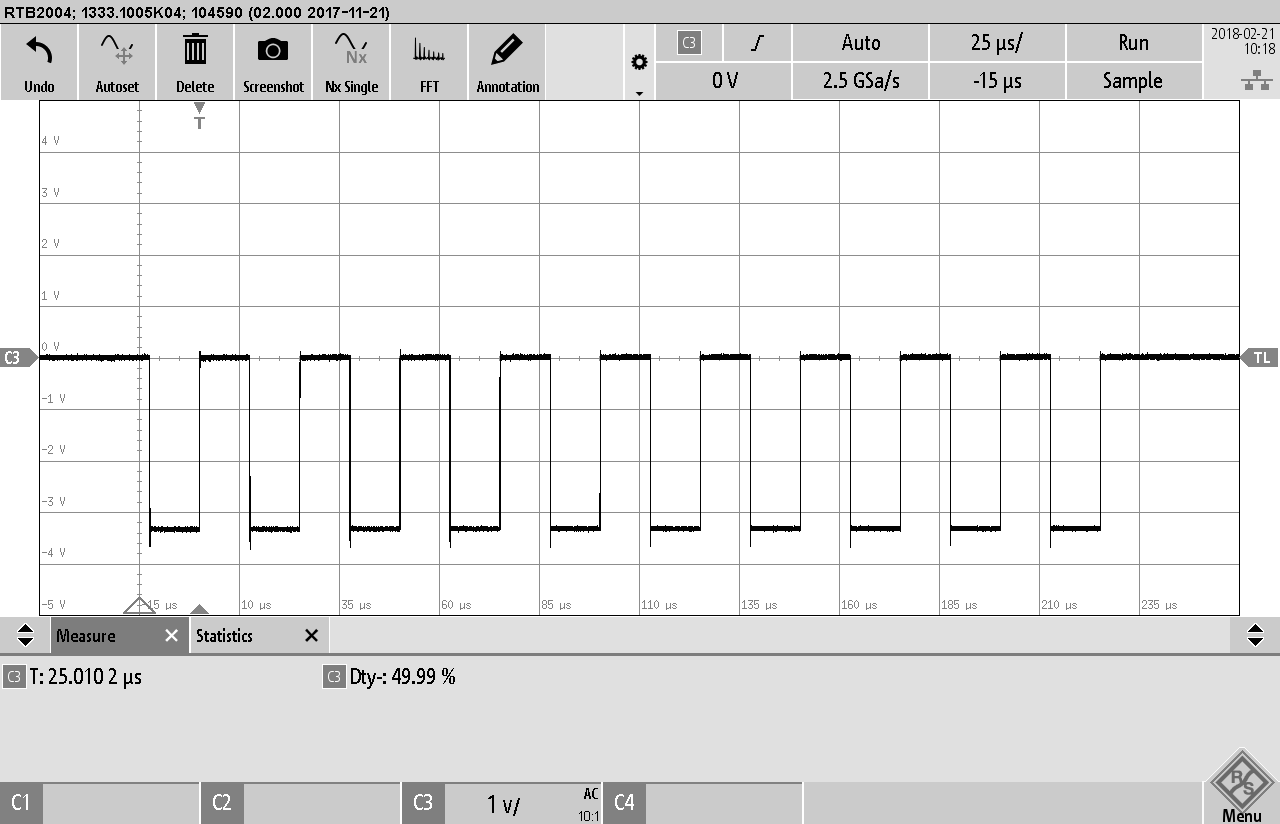
\includegraphics[width=1.0\textwidth]{Abbildungen/PWM-Signal.png}\caption{PWM-Burst auf 40kHz Basis}\label{fig:pwm-burst}
\end{figure}
In der Abbildung \ref{fig:pwm-burst} ist zu sehen, dass ein Burst aus zehn Impulsen mit einer Periodendauer von jeweils 25us generiert wurde. Diese Messung wurde direkt an dem Mikrocontroller vorgenommen, um sicherzustellen dass die H-Brücke mit der passenden Frequenz angesteuert wird.
\begin{figure}[H]
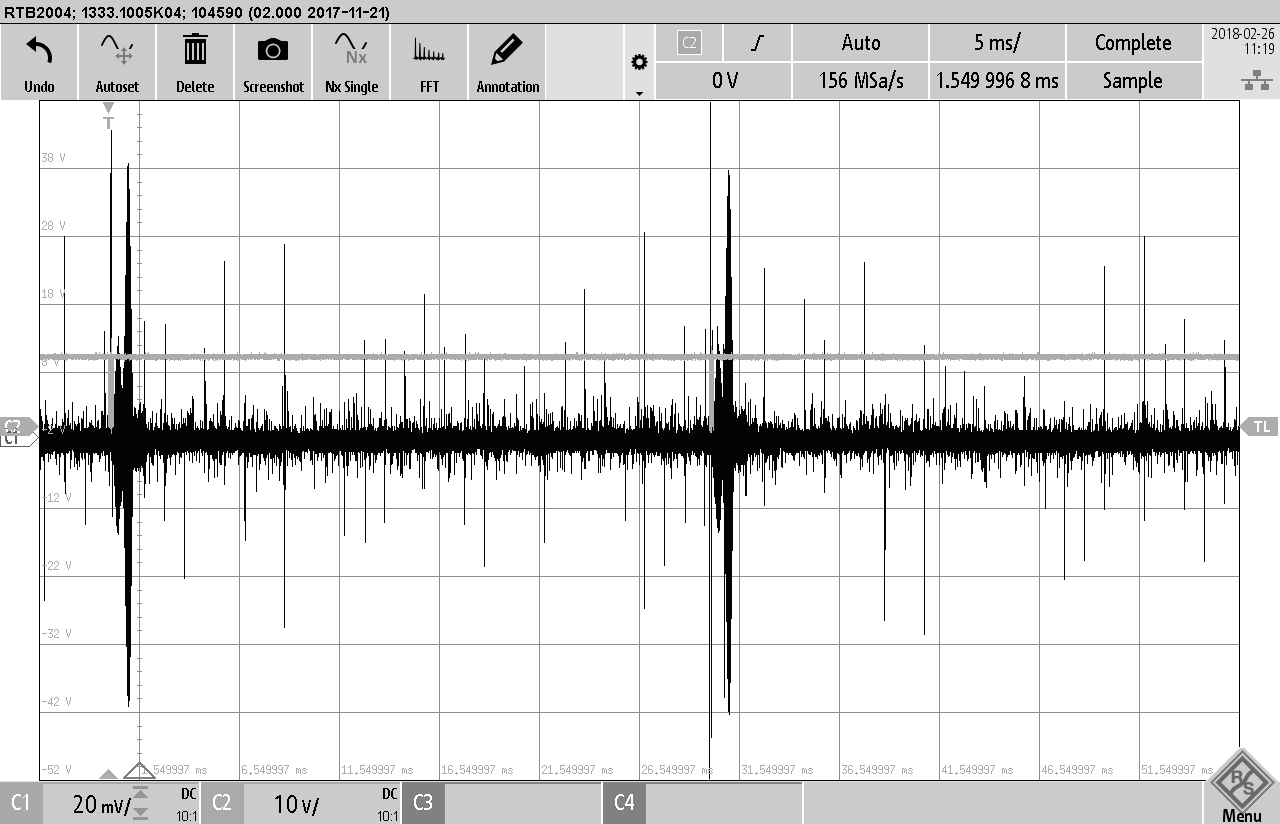
\includegraphics[width=1.0\textwidth]{Abbildungen/Abstand1.png}\caption{Versuchsmessung mit Sender und Empfänger parallel}\label{fig:Abstand1}
\end{figure}
In der Abbildung \ref{Abstand1} ist zu sehen, wie das Eingangssignal am Empfänger aussieht, wenn der Sender und der Empfänger getrennt aufgebaut sind und parallel auf ein Hinderniss gerichtet sind. Dabei zeigt die graue Linie den Verlauf des Sendersignals und die schwarze Linie den Verlauf des Empfängersignals
\section{H-Brücke}
Die H-Brücke wurde durch einen IXDN602, einen MOSFET ersetzt. Dieser wurde als Low-Side Driver-geschaltet. Dies geschah, weil erstens die Beschaltung des OPV nur für eine positive Halbwelle funktioniert und zweitens die Beschaltung der H-Brücke fehlerhaft war. So wurde einer der Ausgänge auf Masse gelegt, was im Betrieb einen Kurzschluss verursachen würde. Um diese Probleme zu beheben, müssten der Sender- und der Empfängerkreis aufgetrennt werden und eine zweite Ultrashallkapsel eingesetzt werden.

\section{Signalverlauf nach Verstärkung durch den OPV}

\section{aufgetretene Probleme}
Zur Inbetriebnahme der H-Brücke mussten Korrekturen vorgenommen werden. Denn diese gab zu Anfang noch keine Signale aus. Es wurde übersehen, dass der OCLSEL-Pin (Oszillatorauswahl) bei der Beschaltung berücksichtigt werden muss. So wurde der Prototyp um eine Drahtbrücke erweitert.
